\documentclass{article}
\usepackage[margin=1in]{geometry}
\usepackage{amsmath}
\usepackage{amssymb}
\usepackage{bm}
\usepackage{pdfpages}
\usepackage{graphicx}
\usepackage{mathtools}
\usepackage{eurosym}
\usepackage[hidelinks]{hyperref}

\usepackage{fancyhdr}
\pagestyle{fancy}
\lhead{Ahou L. -  Ahou S. - Fiorini L. - Portier A.} % controls the left corner of the header
\chead{} % controls the center of the header
\rhead{Groupe 49} % controls the right corner of the header
\lfoot{} % controls the left corner of the footer
\cfoot{} % controls the center of the footer
\cfoot{~\thepage} % controls the right corner of the footer
\usepackage{titlesec}

% Commands for physic unit
\newcommand{\unit}[1]{[\mathrm{#1}]}

\begin{document}

\section*{Question 4A}
Puisque nous nous intéressons seulement aux bilans de productions/consommations et du niveau du bassin
sur des périodes de $T \unit{h}$, nous pouvons exprimer toutes nos variables en fonction de cette période.\\
Voici deux tableaux reprenant les notations principales utilisées dans cette seconde partie \footnote{Toutes autres notations utilisées dans la suite seront définies lorsque celles-ci seront introduites} : 

\begin{table}[h!]
    \centering
    \renewcommand{\arraystretch}{1.5}% Add spacing between rows : default value is 1
    \begin{tabular}{|c || c |} 
        \hline
        Nom & Signification\\
        \hline\hline
        $c_i$ & Capacité éolienne installée sur le i\textsuperscript{ème} site\\
        $t_j$ & Puissance de turbinage choisie durant la j\textsuperscript{ème} période\\
        $p_j$ & Puissance de pompage choisie durant la j\textsuperscript{ème} période\\
        \hline
    \end{tabular}
    \caption{Table des notations des variables de décisions utilisées pour le modèle de la question 4.}
    \label{table:notations_variables_4}
\end{table}

\begin{table}[h!]
    \centering
    \renewcommand{\arraystretch}{1.5}% Add spacing between rows : default value is 1
    \begin{tabular}{|c || p{14cm} |} 
        \hline
        Nom & Signification\\
        \hline\hline
        $n$ & Nombre de sites éoliens \\
        $m$ & Nombre de périodes de $T \unit{h}$ dans une année\\
        $e_i(j)$ & Rendement éolien du i\textsuperscript{ème} site durant la j\textsuperscript{ème} période\\
        $a_j$ & Apport fluvial durant la j\textsuperscript{ème} période\\
        $\mathrm{cons}_j$ & Consommation énergétique durant la j\textsuperscript{ème} période\\
        $t_\mathrm{max}$ & Capacité maximale de turbinage\\
        $p_\mathrm{max}$ & Capacité maximale de pompage\\
        $\mathrm{stock}_\mathrm{max}$ & Capacité de stockage maximale\\
        $\eta$ & Rendement de turbinage\\
        $\mathrm{costs}$ & Vecteur donnant les valeurs du coût d'installation d'un site éolien  (onshore/offshore) \newline $\mathrm{costs}_i = $ Coût d'installation d'un site onshore si le site d'index $i$ est onshore, et inversement.\\  
        \hline
    \end{tabular}
    \caption{Table des notations des constantes utilisées pour le modèle.}
    \label{table:notations_constantes}
\end{table}

\noindent
Le modèle peut alors s'écrire ainsi :
\begin{align}
    \min_{c_{i},t_j,p_j} \quad &\mathrm{costs}^\intercal\mathbf{c} \nonumber\\
    \textrm{tel que} \quad & \sum_{i=0}^{n-1} c_i e_i(j) + \eta \cdot t_j - p_j \ge \mathrm{cons}_j \quad \forall j \in  \{ 0, \ldots, m-1 \}\label{eq:4A_contr1}\\
    & 0 \le \frac{\mathrm{stock}_\mathrm{max}}{2}  + \sum_{j=0}^{k} p_j - t_j + a_j \le  \mathrm{stock}_\mathrm{max} \quad \forall k \in \{ 0, \ldots, m-2 \}\label{eq:4A_contr2}\\
    & \sum_{j=0}^{m-1} p_j - t_j + a_j = 0 \label{eq:4A_contr3}\\
    & 0 \le c_i \le c_i^\mathrm{max} \quad \forall i \in  \{ 0, \ldots, n-1 \}  \label{eq:4A_contr4}\\
    & 0 \le t_j \le T \cdot t_\mathrm{max} \quad \forall j \in  \{ 0, \ldots, m-1 \}  \label{eq:4A_contr5}\\
    & 0 \le p_j \le T \cdot p_\mathrm{max} \quad \forall j \in  \{ 0, \ldots, m-1 \} \label{eq:4A_contr6}
\end{align}

\newpage

La fonction objectif représente le coût d'installation des éoliennes (en tenant compte des différences entre les installations \textit{offshore} et \textit{onshore}). 
Cela revient au même que de minimiser le prix moyen de l'énergie consomée car il suffit de diviser le coût total de l'installation par la demande totale en énergie qui est une constante.\\
La contrainte \eqref{eq:4A_contr1} indique qu'il faut satisfaire la demande en énergie en fin de chaque période de $T \unit{h}$ en tenant compte de la production éolienne
ainsi que des opérations de turbinage/pompage.\\
La contrainte \eqref{eq:4A_contr2} fait le bilan lié aux variations des opérations de turbinage/pompage décidées et de l'apport fluvial naturel depuis le temps $t = 0$ jusqu'en tout temps $t = k$ afin de calculer l'augmentation/la diminution du niveau de l'eau dans le bassin.\\
La formalisation peut s'obtenir en sachant que le niveau initial de notre bassin est à $0.5 \times \mathrm{stock}_\mathrm{max}$, puis que le niveau du bassin au prochain temps est le niveau du bassin passé plus les fluctuations à la période $j$, pompage - turbinage + apport fluvial, qui est donné plus formellement par $\mathrm{bassin}_{j+1} = \mathrm{bassin}_{j} + p_j - t_j + a_j$, donc en développant cette relation de récurrence, nous obtenons 
bien le niveau de notre bassin pour toute période $j \in \{ 0, \ldots, m-1 \}$ en fonction de nos variables, et en sachant que le niveau du bassin doit revenir à son niveau initial, à la fin 
de la période considérée, il y a une contrainte "en moins" pour \eqref{eq:4A_contr2} qui apparaît dans \eqref{eq:4A_contr3}. \\
La contrainte \eqref{eq:4A_contr3} indique que le niveau final du bassin doit revenir au même niveau qu'initialement. Autrement dit, les opérations de turbinage/pompage et 
l'apport fluvial doivent se sommer à 0 à la fin de la dernière période.\\
Les contraintes \eqref{eq:4A_contr4}, \eqref{eq:4A_contr5} et \eqref{eq:4A_contr6} indiquent respectivement les bornes sur les capacités éoliennes maximales installables sur chaque site, 
les capacités maximales de turbinages et les capacités maximales de pompages pour des périodes de $T \unit{h}$, regroupées au niveau européen, bien entendu.

\newpage % Car il faudra rendre sur Gradescope en séparant les questions

\section*{Question 4B}
Suite à l'implémentation de notre problème d'optimisation sur le notebook Jupyter, nous obtenons 
un coût minimum moyen (car nous avons simplement divisé par le nombre de périodes (8960/3 = 2920 périodes de 3 heures)
) par période qui est d'environ $67.947.438,96$\euro, nous pouvons obtenir le coût total sur un an qui est donné par 
$67.947.438,96 * 2.920$\euro $= 198.406.521.770,2$\euro, nous avons alors finalement en divisant par la demande totale,
un coût de $76,6$\euro /MWh  \footnote{C'est une valeur qui semble cohérente, surtout pour un modèle comme ici, 
assez libre et qui ne prétend pas refléter les réalités, le prix moyen de l'énergie par MWh en Europe actuellement 
est aux alentours de quelques centaines d'euros, d'après la Commission européenne : 
\url{https://ec.europa.eu/eurostat/statistics-explained/index.php?title=Electricity_price_statistics}, 
consulté le 8 mai 2024 à 01h08.}.


\begin{figure}[h!]
    \centering
    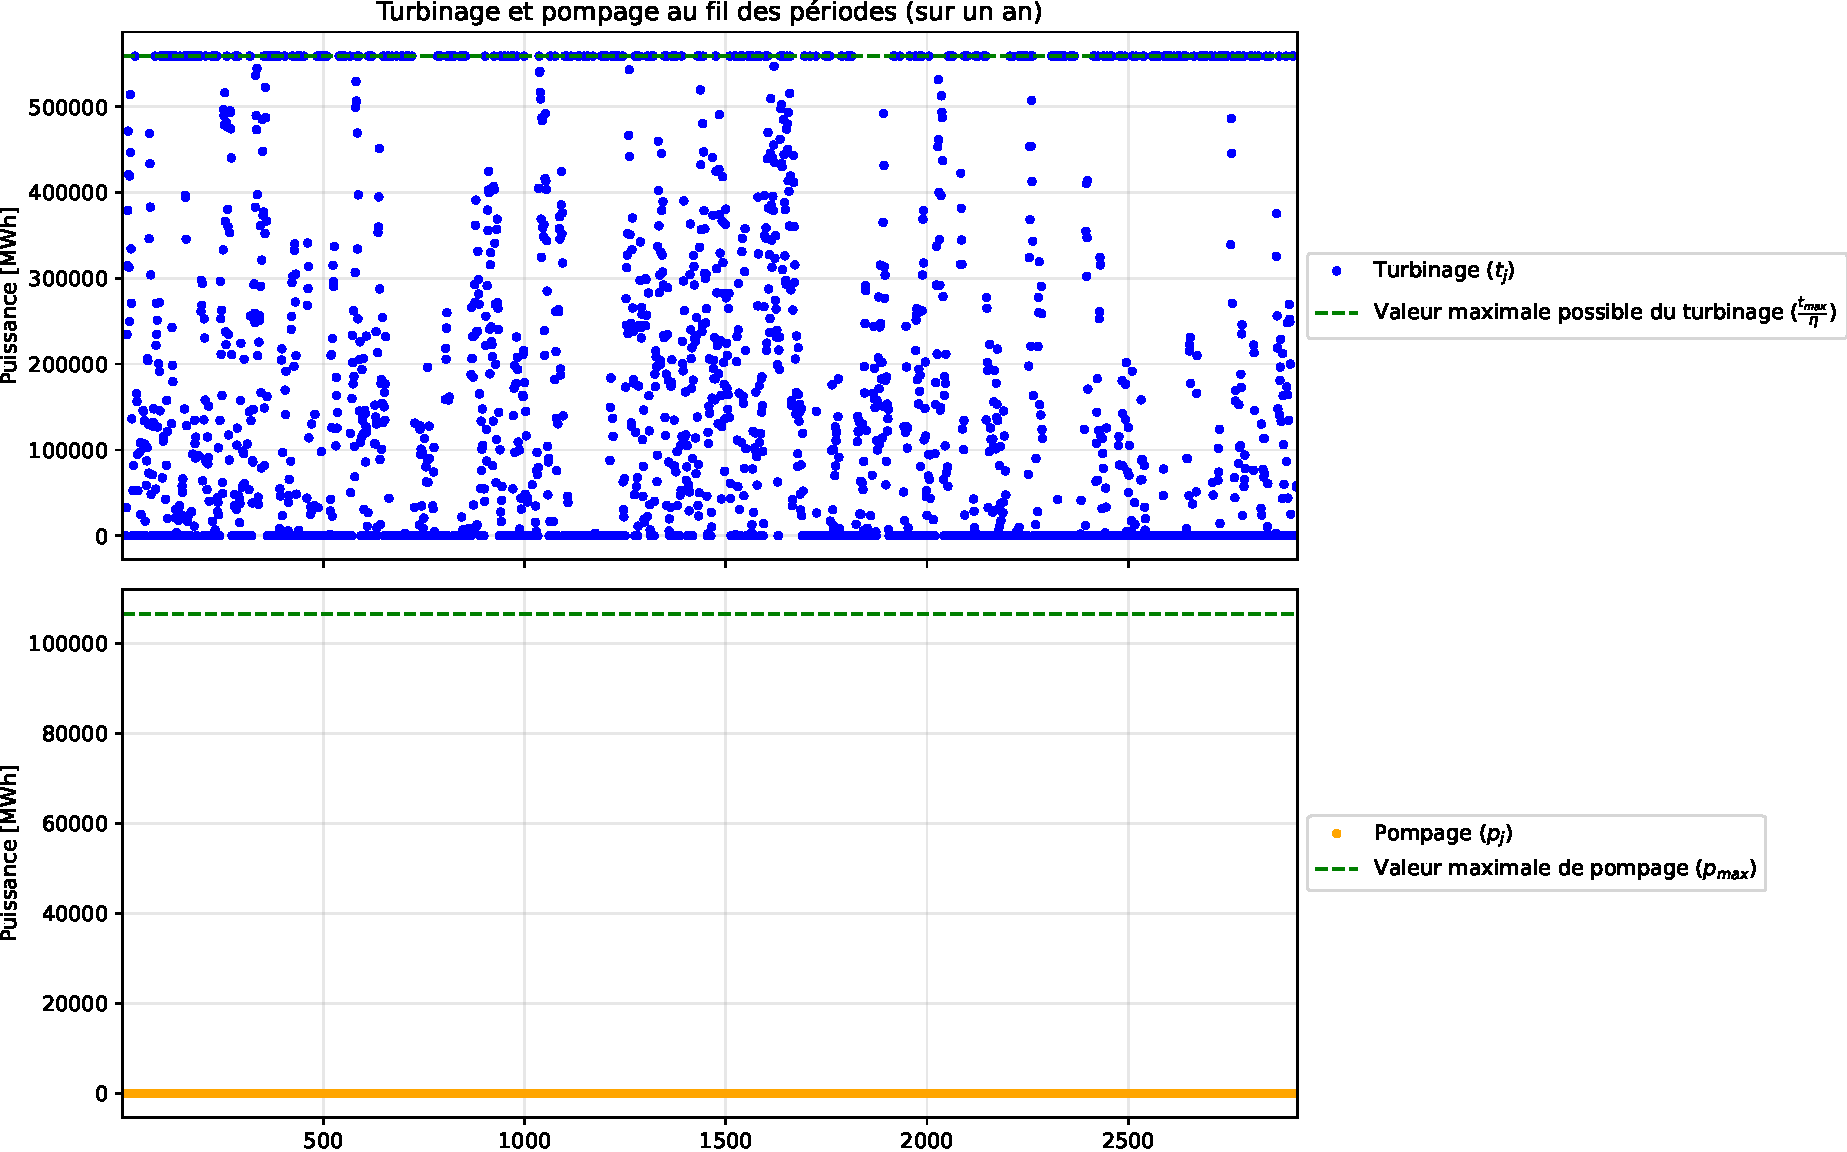
\includegraphics[scale=0.6]{GraphesP2/Turbinage_pompage_Q4.pdf}
    \caption{Test}
    \label{fig:Turbinage_pompage_Q4}
\end{figure}
\begin{figure}[h!]
    \centering
    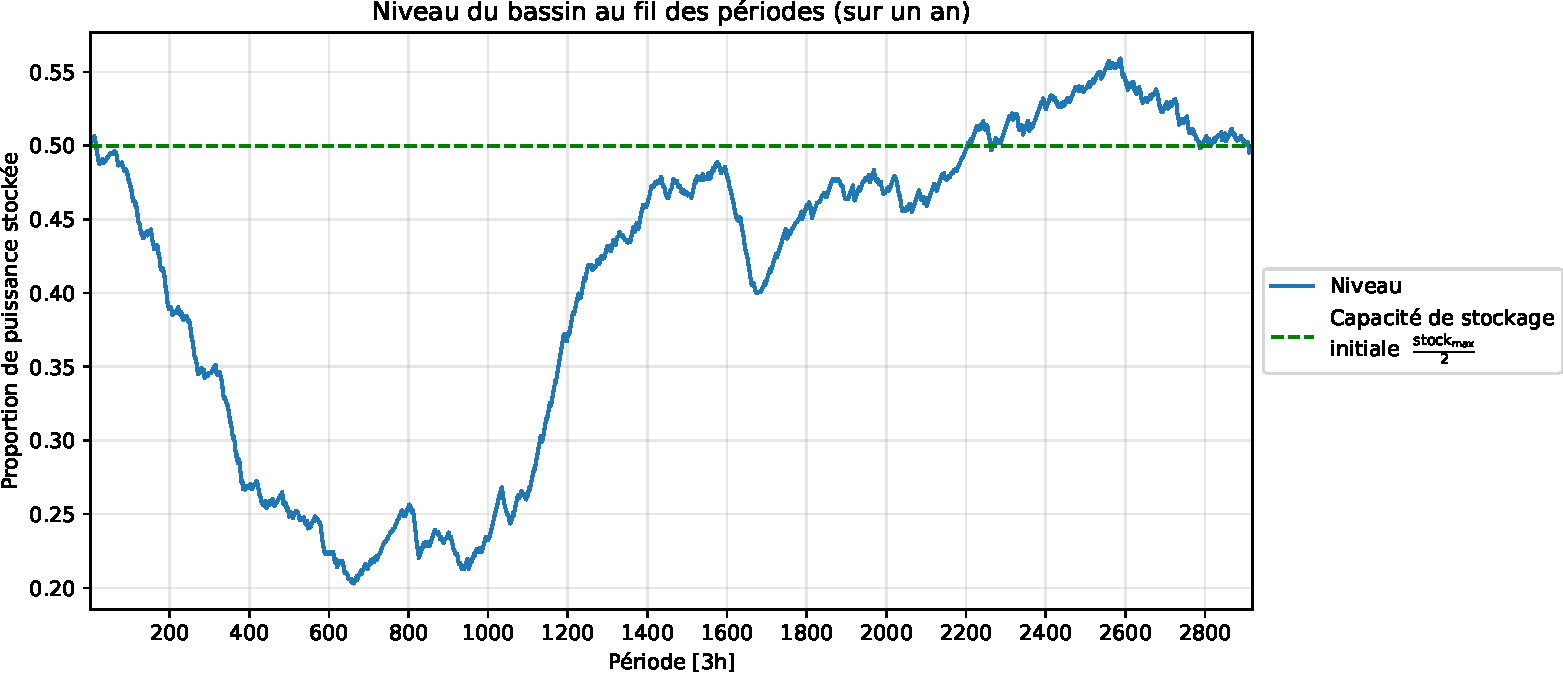
\includegraphics[scale=0.6]{GraphesP2/Niveau_Bassin_Q4.pdf}
    \caption{Test}
    \label{fig:Niveau_bassin_Q4}
\end{figure}
\begin{figure}[h!]
    \centering
    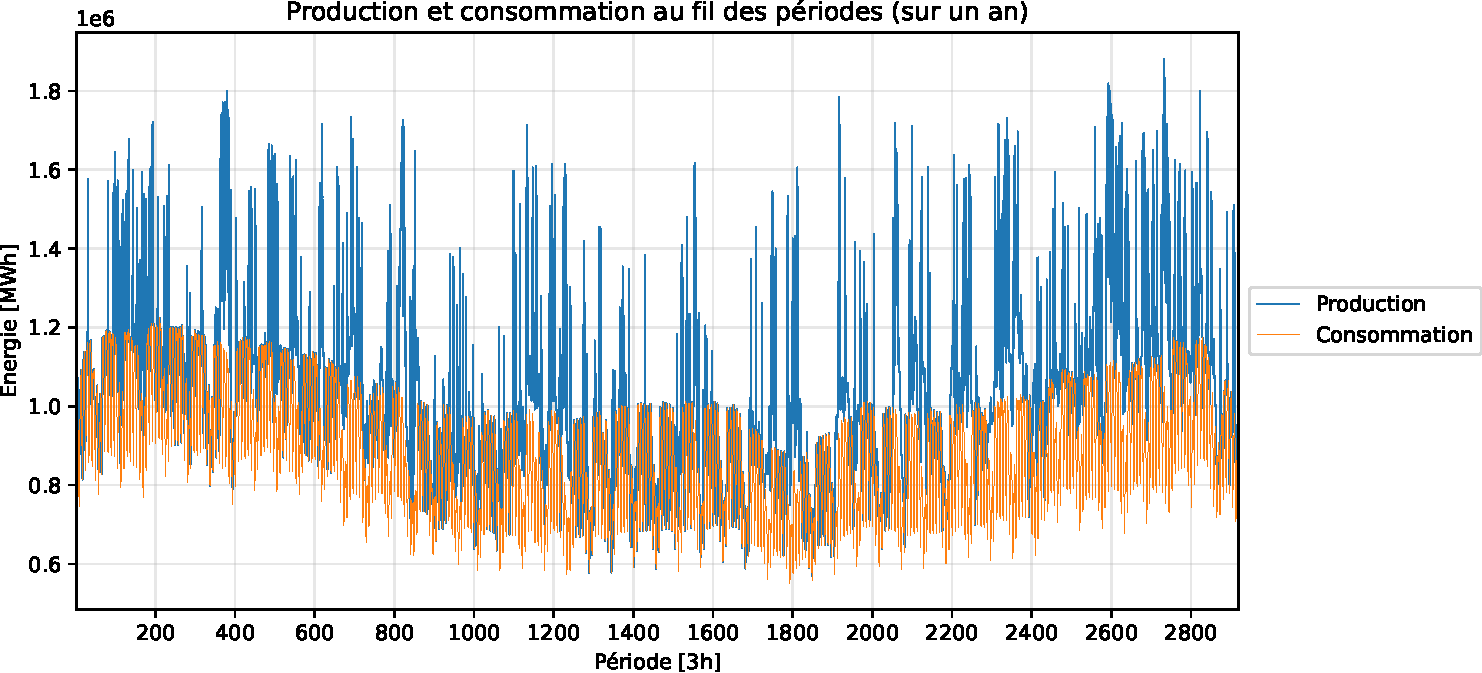
\includegraphics[scale=0.6]{GraphesP2/Prod_Cons_Q4.pdf}
    \caption{Test}
    \label{fig:Prod_Cons_Q4}
\end{figure}


\clearpage
\section*{Question 4C}

\newpage
\section*{Question 5}
Nous devons à présent choisir, pour chaque site d'éoliennes, si nous installons $0\%, 50\%$ ou $100\%$ de la capacité maximale installable sur ce site.
Pour ce faire, nous rédéfinissons les variables $c_i$ de la question 4 :

\begin{table}[h!]
    \centering
    \renewcommand{\arraystretch}{1.5}% Add spacing between rows : default value is 1
    \begin{tabular}{|c || c |} 
        \hline
        Nom & Signification\\
        \hline\hline
        $c_{i} \in \{ 0, 1, 2 \}$ & Proportion de la capacité maximale $c_i^\mathrm{max}$ installée sur le i\textsuperscript{ème} site\\
        $t_j$ & Puissance de turbinage choisie durant la j\textsuperscript{ème} période\\
        $p_j$ & Puissance de pompage choisie durant la j\textsuperscript{ème} période\\
        \hline
    \end{tabular}
    \caption{Table des nouvelles notations des variables de décisions utilisées pour le modèle de la question 5.}
    \label{table:notations_variables_5}
\end{table} 
\noindent La puissance installée sur le i\textsuperscript{ème} site équivaut alors à $0.5 \cdot c_ic_i^\mathrm{max}$. Le modèle devient alors :
\begin{align}
    \min_{c_{i} \in \mathbb{Z},t_j,p_j} \quad &\mathrm{costs}^\intercal 
    \begin{pmatrix}
        c_0c_0^\mathrm{max}\\
        \vdots\\
        c_{n-1}c_{n-1}^\mathrm{max}
    \end{pmatrix} \nonumber\\
    \textrm{tel que} \quad & \sum_{i=0}^{n-1} 0.5 \cdot c_ic_i^{max} e_i(j) + \eta \cdot t_j - p_j \ge \mathrm{cons}_j \quad \forall j \in  \{ 0, \ldots, m-1 \}\label{eq:5_contr1}\\
    & 0 \le \frac{\mathrm{stock}_\mathrm{max}}{2}  + \sum_{j=0}^{k} p_j - t_j + a_j \le  \mathrm{stock}_\mathrm{max} \quad \forall k \in \{ 0, \ldots, m-2 \}\label{eq:5_contr2}\\
    & \sum_{j=0}^{m-1} p_j - t_j + a_j = 0 \label{eq:5_contr3}\\
    & 0\le c_i \le 2 \quad \forall i \in  \{ 0, \ldots, n-1 \} \label{eq:5_contr4}  \\
    & 0 \le t_j \le T \cdot t_\mathrm{max} \quad \forall j \in  \{ 0, \ldots, m-1 \} \label{eq:5_contr5}\\
    & 0 \le p_j \le T \cdot p_\mathrm{max} \quad \forall j \in  \{ 0, \ldots, m-1 \} \label{eq:5_contr6} 
\end{align}

\noindent Après résolution du problème, nous obtenons seulement une légère différence quant au prix moyen de l'énergie.
Celui-ci passe d'une valeur de $76.6$\euro/MWh à $76.62$\euro/MWh. Bien que cela puisse sembler un peu faible, nous constatons
une différence de coût total entre la question 5 et la question 4 qui est de $55.249.753,95$ \euro, donc
la restriction à 3 cas des $c_i$ nous coûte plus cher de 55 millions d'euros, cependant, dans un cas réel, cela
pourrait nous être avantageux, car bien que les $c_i^\mathrm{max}$ varient, il serait peut-être possible
de faire des économies d'échelle sur l'installation des sites en imaginant trois configurations possibles en fonction
des ordres de grandeur des $c_i^\mathrm{max}$. 


\end{document}
